% Class Notes Template
\documentclass[12pt]{article}
\usepackage[margin=1in]{geometry} 
\usepackage[utf8]{inputenc}

% Packages
\usepackage[french, english]{babel}
\usepackage{amsmath, amsthm, amssymb ,amsfonts, graphics, tikz, float, enumerate}
\usepackage{listings}
\usepackage{color} %red, green, blue, yellow, cyan, magenta, black, white
\definecolor{mygreen}{RGB}{28,172,0} % color values Red, Green, Blue
\definecolor{mylilas}{RGB}{170,55,241}

\lstset{language=Matlab,%
	%basicstyle=\color{red},
	breaklines=true,%
	morekeywords={matlab2tikz},
	keywordstyle=\color{blue},%
	morekeywords=[2]{1}, keywordstyle=[2]{\color{black}},
	identifierstyle=\color{black},%
	stringstyle=\color{mylilas},
	commentstyle=\color{mygreen},%
	showstringspaces=false,%without this there will be a symbol in the places where there is a space
	numbers=left,%
	numberstyle={\tiny \color{black}},% size of the numbers
	numbersep=9pt, % this defines how far the numbers are from the text
	emph=[1]{for,end,break},emphstyle=[1]\color{blue}, %some words to emphasise
	%emph=[2]{word1,word2}, emphstyle=[2]{style},    
}

% Title
\title{ECON 6130 - Problem Set \# 5}
\date{\today}
\author{Julien Manuel Neves}

% Use these for theorems, lemmas, proofs, etc.
\theoremstyle{definition}
\newtheorem{example}{Example}[section]
\newtheorem{theorem}{Theorem}
\newtheorem{lemma}[theorem]{Lemma}
\newtheorem{proposition}[theorem]{Proposition}
\newtheorem{claim}[theorem]{Claim}
\newtheorem{axiom}[theorem]{Axiom}
\newtheorem{corollary}[theorem]{Corollary}
\newtheorem{remark}[theorem]{Remark}
\newtheorem{definition}[theorem]{Definition}

% Usefuls Macros
\newcommand\N{\mathbb{N}}
\newcommand\E{\mathbb{E}}
\newcommand\R{\mathbb{R}}
\newcommand\F{\mathcal{F}}
\newcommand\Z{\mathbb{Z}}
\newcommand\st{\text{ such that }}
\newcommand\seq[1]{\{ #1 \}}
\newcommand{\inv}{^{-1}}

\newcommand{\pa}[1]{\left(#1\right)}
\newcommand{\bra}[1]{\left[#1\right]}
\newcommand{\cbra}[1]{\left\{#1\right\}}

\newcommand{\pfrac}[2]{\pa{\frac{#1}{#2}}}
\newcommand{\bfrac}[2]{\bra{\frac{#1}{#2}}}

\newcommand{\mat}[1]{\begin{matrix}#1\end{matrix}}
\newcommand{\pmat}[1]{\pa{\mat{#1}}}
\newcommand{\bmat}[1]{\bra{\mat{#1}}}


\begin{document}

\maketitle

\section*{Problem 1}

\begin{enumerate}[1.]
	\item 
	\underline{Sequential problem}
	\begin{align*}
		\max &\sum_{t=0}^{\infty} \beta^t u(C_t) \\
		 \st & C_t = F(K_{C,t}, L_{C,t})\\
		 & I_t = G(K_{I,t}, L_{I,t})\\
		 & I_t = I_{C,t}+ I_{I,t}\\
		 & L = L_{C,t}+ L_{I,t}\\
		 & K_{C,t+1} = (1-\delta) K_{I,t} + I_{I,t}\\
		 & K_{I,t+1} = (1-\delta) K_{C,t} + I_{C,t}\\
		 & \text{where }L, K_{C,0} \text{ and } K_{I,0} \text{ given.}
	\end{align*}
	
	Note that we can write $K_{I,t+1}$ in the following way
	\[
	K_{I,t+1} = (1-\delta)(K_{C,t}+K_{I,t})+G(K_{I,t}, L-L_{C,t})-K_{C,t+1}
	\]
	
	\underline{Recursive problem}
		\begin{align*}
	V( K_{C,t}, K_{I,t} ) = \max_{L_{C,t}, K_{C,t+1}}  & \left\lbrace u( F(K_{C,t},L_{C,t})) \right.  \\
	&\left. + \beta V(K_{C,t+1}, (1-\delta)(K_{C,t}+K_{I,t})+G(K_{I,t}, L-L_{C,t})-K_{C,t+1})\right\rbrace
	\end{align*}
	where
	\begin{enumerate}[(i)]
		\item Control variables.
		\[
		L_{C,t} \text{ and } K_{C,t+1}
		\]
		\item State variables.
		\[
		K_{C,t} \text{ and } K_{I,t}
		\]
	\end{enumerate}


	\item 
	
	
	\begin{enumerate}[(1)]
		\item First-Order conditions.
		
		\begin{enumerate}[(i)]
			\item $K_{C,t+1}$
			\begin{align*}
				&\beta V_1(K_{C,t+1}, (1-\delta)(K_{C,t}+K_{I,t})+G(K_{I,t}, L-L_{C,t})-K_{C,t+1})\\ -& \beta V_2(K_{C,t+1}, (1-\delta)(K_{C,t}+K_{I,t})+G(K_{I,t}, L-L_{C,t})-K_{C,t+1}) = 0\\
				\Rightarrow & V_1(K_{C,t+1},K_{I,t+1}) = V_2(K_{C,t+1},K_{I,t+1}) 
			\end{align*}
			\item $L_{C,t}$
			
			\begin{align*}
			& u'(F(K_{C,t},L_{C,t})) F_2(K_{C,t},L_{C,t})\\
			- &\beta V_2(K_{C,t+1}, (1-\delta)(K_{C,t}+K_{I,t})+G(K_{I,t}, L-L_{C,t})-K_{C,t+1}) G_2(K_{I,t}, L-L_{C,t})= 0\\
			\Rightarrow & u'(C_t) F_2(K_{C,t},L_{C,t}) = \beta V_2(K_{C,t+1},K_{I,t+1}) G_2(K_{I,t}, L_{I,t})
			\end{align*}
		\end{enumerate}
		
		\item Envelope conditions.
		
		Let  $X_{j,t}^*$ be the choice of $X_{j,t}$ according to the policy function.
		\begin{enumerate}[(i)]
			\item $K_{C,t}$
			\begin{align*}
			& V_1(K_{C,t},K_{I,t}) = u'(F(K_{C,t},L_{C,t}^*)) F_1(K_{C,t},L_{C,t}^*) \\
			 +&  \beta\left\lbrace  V_2(K_{C,t+1}^*,(1-\delta)(K_{C,t}+K_{I,t})+G(K_{I,t}, L-L_{C,t}^*)-K_{C,t+1}^*)(1-\delta)\right\rbrace \\
			 \Rightarrow & V_1(K_{C,t},K_{I,t})	= u'({C_t}^*)) F_1(K_{C,t},L_{C,t}^*)	+ \beta V_2(K_{C,t+1}^*,K_{I,t+1}^*)(1-\delta)	
			\end{align*}
			\item $K_{I,t}$
			\begin{align*}
			V_2(K_{C,t},K_{I,t}) = \beta & \left\lbrace  V_2(K_{C,t+1}^*,(1-\delta)(K_{C,t}+K_{I,t})+G(K_{I,t}, L-L_{C,t}^*)-K_{C,t+1}^*)\right. \\
			& \times  \left.    (1-\delta + G_1(K_{I,t}, L-L_{C,t}^*))\right\rbrace \\
			\Rightarrow  V_2(K_{C,t},K_{I,t})	& = \beta V_2(K_{C,t+1}^*,K_{I,t+1}^*)(1-\delta + G_1(K_{I,t}, L_{I,t}^*))		
			\end{align*}
			
		\end{enumerate}
	
	\end{enumerate}

	\item 
	
	Let $X_{j}  = X_{j,t}= X_{j,t+1}$, where $j = \cbra{ C,I, \emptyset}$ and $X = \cbra{K,L,C}$.
	
	Note that in the steady state we have $X_j^*=X_j$ and
	\begin{align*}
		K_I+K_C&=\frac{G(K_I,L_I)}{\delta} \\
		L_I+L_C &=L
	\end{align*}
	Then, combining the first-order and envelope conditions, we get
	\begin{align*}
		V_1(K_C,K_I) & = V_2(K_C,K_I) \\
		u'(C) F_2(K_{C},L_{C}) &= \beta V_2(K_{C},K_{I}) G_2(K_{I}, L_{I})\\
		V_1(K_{C},K_{I})	&= u'({C})) F_1(K_{C},L_{C})	+ \beta V_2(K_{C},K_{I})(1-\delta)\\
		V_2(K_{C},K_{I})	& = \beta V_2(K_{C},K_{I})(1-\delta + G_1(K_{I}, L_{I}))
	\end{align*}
	where $K_I =\frac{G(K_I,L_I)}{\delta} -K_C$ and $L_I = L - L_C$.
	
	This reduce to the following system of equations
	\begin{align*}
	\frac{1}{\beta}	&= 1-\delta +\frac{ G_2(K_{I}, L_{I})}{F_2(K_{C},L_{C})} F_1(K_{C},L_{C})	\\
	\frac{1}{\beta}	& = 1-\delta + G_1(K_{I}, L_{I})
	\end{align*}
	where $K_I =\frac{G(K_I,L_I)}{\delta} -K_C$ and $L_I = L - L_C$.
	\item 
	
	We can take the previous equations to derive the following
	\begin{align*}
	\Rightarrow \frac{ G_2(K_{I}, L_{I})}{F_2(K_{C},L_{C})} F_1(K_{C},L_{C}) & = G_1(K_{I}, L_{I})\\
	\frac{ G_2(K_{I}, L_{I})}{G_1(K_{C},L_{C})}& = \frac{ F_2(K_{I}, L_{I})}{F_1(K_{C},L_{C})}\\
	\frac{ (1-\gamma)K_{I}^{\gamma}L_{I}^{-\gamma} }{ \gamma K_{I}^{\gamma-1}L_{I}^{1-\gamma} }& = \frac{ (1-\alpha)K_{C}^{\alpha}L_{C}^{-\alpha} }{ \alpha K_{C}^{\alpha-1}L_{C}^{1-\alpha} }\\
	\frac{(1-\gamma)}{\gamma}\frac{ K_{I}}{L_{I}}& = \frac{(1-\alpha)}{\alpha}\frac{ K_{C}}{L_{C}}
	\end{align*}
	
	Additionally,
		\begin{align*}
	\frac{1}{\beta}	& = 1-\delta + G_1(K_{I}, L_{I}) \\
	\frac{1}{\beta}	& = 1-\delta + \gamma K_{I}^{\gamma-1}L_{I}^{1-\gamma} \\
	\frac{1}{\beta}	& = 1-\delta + \gamma \left( \frac{K_{I}}{L_{I}}\right) ^{\gamma-1} \\
	\Rightarrow \frac{K_{I}}{L_{I}} & =\left(\frac{\gamma}{\frac{1}{\beta}-1+\delta} \right)^{\frac{1}{1-\gamma}}\\
	\Rightarrow \frac{K_{C}}{L_{C}} & =\frac{\alpha(1-\gamma)}{\gamma(1-\alpha)} \left(\frac{\gamma}{\frac{1}{\beta}-1+\delta} \right)^{\frac{1}{1-\gamma}}
	\end{align*}
	
	Then, we can solve for $L_C$ in the following way
	\begin{align*}
	K_I & =\frac{G(K_I,L_I)}{\delta} -K_C \\
	\frac{K_I}{L_I} & = \left( \frac{K_I}{L_I}\right)^\gamma  \frac{1}{\delta} -\frac{K_C}{L_I} \\
	\frac{K_I}{L_I} & = \left( \frac{K_I}{L_I}\right)^\gamma  \frac{1}{\delta} -\frac{K_C}{L_C}\frac{L_C}{(1-L_C)} \\
	\left(\frac{\gamma}{\frac{1}{\beta}-1+\delta} \right)^{\frac{1}{1-\gamma}} & = \left(\frac{\gamma}{\frac{1}{\beta}-1+\delta} \right)^{\frac{\gamma}{1-\gamma}}  \frac{1}{\delta} -\frac{\alpha(1-\gamma)}{\gamma(1-\alpha)} \left(\frac{\gamma}{\frac{1}{\beta}-1+\delta} \right)^{\frac{1}{1-\gamma}}\frac{L_C}{(L-L_C)} \\
	 \frac{L_C}{(L-L_C)} & =\frac{\gamma(1-\alpha)}{\alpha(1-\gamma)}\left( \frac{1}{\delta}\left(\frac{\frac{1}{\beta}-1+\delta}{\gamma} \right)-1\right)
	\end{align*}
	
	Let $ \Delta =\frac{\gamma(1-\alpha)}{\alpha(1-\gamma)}\left( \frac{1}{\delta}\left(\frac{\frac{1}{\beta}-1+\delta}{\gamma} \right)-1\right) $, then
	\begin{align*}
		L_C &= \frac{\Delta}{1+\Delta}L\\
		L_I &= \frac{1}{1+\Delta}L\\
		K_C &=  \frac{\alpha(1-\gamma)}{\gamma(1-\alpha)} \left(\frac{\gamma}{\frac{1}{\beta}-1+\delta} \right)^{\frac{1}{1-\gamma}} \frac{\Delta}{1+\Delta}L\\
		K_I &=  \left(\frac{\gamma}{\frac{1}{\beta}-1+\delta} \right)^{\frac{1}{1-\gamma}} \frac{1}{1+\Delta}L
	\end{align*}
	
	
\end{enumerate}

\section*{Problem 2}

\begin{enumerate}[1.]
	\item 
	
	\underline{Recursive problem}
	\begin{align*}
	V( k_{t}, y_t) & = \max_{0\leq  k_{t+1} \leq e^yk_t^\alpha + (1-\delta)k_t}   \left\lbrace u( e^yk_t^\alpha +  (1-\delta)k_t - k_{t+1}) + \beta \sum_{y_{t+1}} \pi(y_{t+1}\mid y_t) V(k_{t+1},y_{t+1})\right\rbrace \\
	&\text{where } k_0, y_0 \text{ given}
	\end{align*}
	where $\pi(y_{t+1}\mid y_t) = Prob(y=y_{t+1}\mid y=y_t)$ and
	\begin{enumerate}[(i)]
	\item Control variables.
	\[
	k_{t+1}
	\]
	\item State variables.
	\[
	k_{t} \text{ and } y_{t}
	\]
\end{enumerate}
	
	Note that $0\leq  k_{t+1} \leq e^yk_t^\alpha + (1-\delta)k_t$ is a non-empty, compact, continuous, convex and monotone set.
	
	Thus, for $V(\cdot)$ to be continuous, monotone and concave, we need the following assumptions on $u(\cdot)$:
	\begin{enumerate}
		\item Continuous and bounded
		\item Strictly increasing in $c_t$
		\item Strictly concave
	\end{enumerate}
	
	\item 
	
	Note that the code is given in the appendix.
	
	Figure \ref{fig:plotmarkov} gives the sample distribution of 10000 replications of a 1000 period Markov chain.
	\begin{figure}[H]
		\centering
		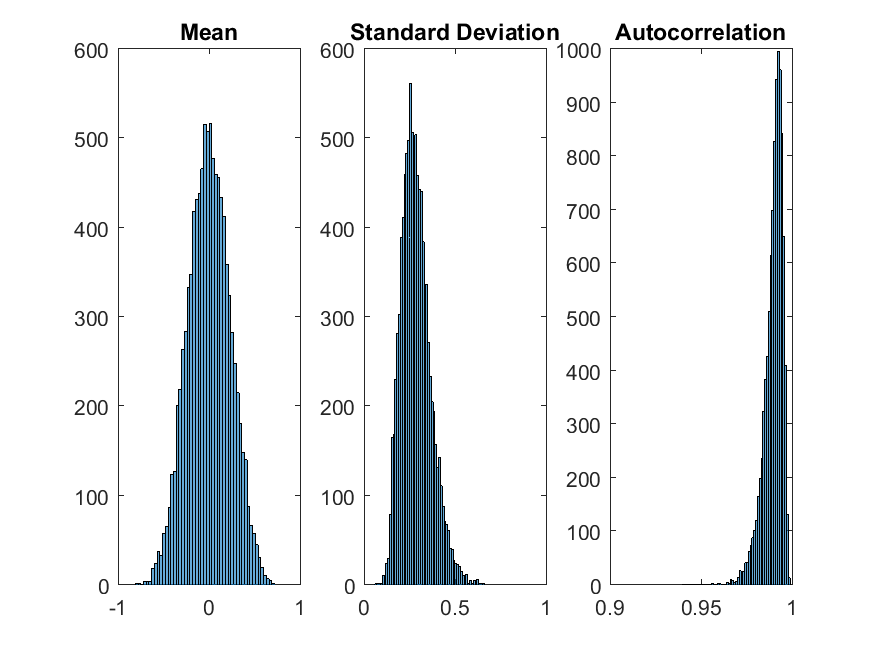
\includegraphics[width=\linewidth]{plot_markov}
		\caption{Distribution of Markov Chain}
		\label{fig:plotmarkov}
	\end{figure}

\begin{enumerate}[(i)]
	\item Mean: 0.0003    
	\item Standard Deviation: 0.2867    
	\item Autocorrelation: 0.9898
\end{enumerate}


\item 

\underline{Policy function}
\begin{figure}[H]
	\centering
	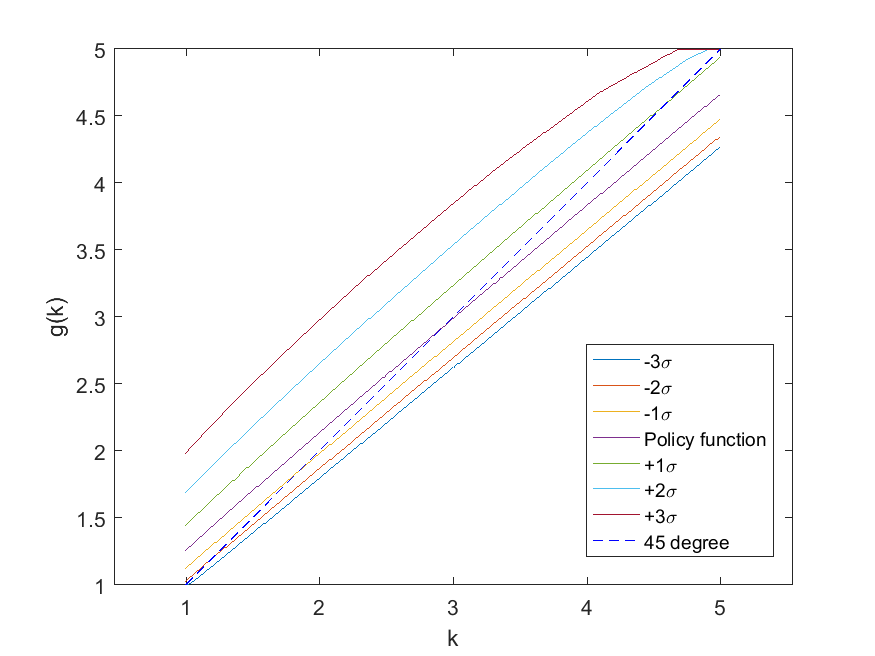
\includegraphics[width=\linewidth]{plot_policy}
	\caption{Policy Function}
	\label{fig:plotpolicy}
\end{figure}

\underline{Value function}
\begin{figure}[H]
	\centering
	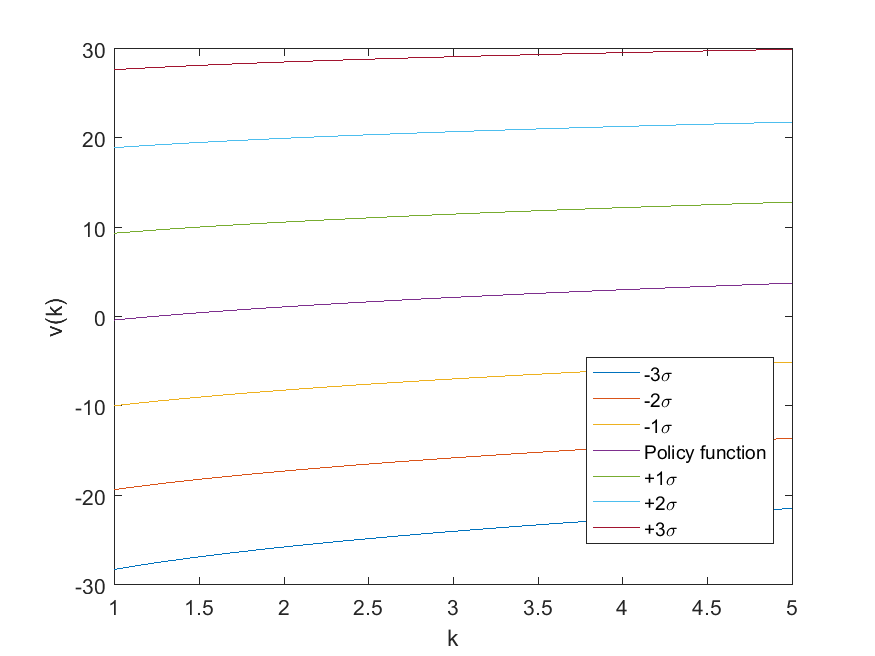
\includegraphics[width=\linewidth]{plot_value}
	\caption{Value Function}
	\label{fig:plotvalue}
\end{figure}

\item 
	
	 The simulation is terrible! As we can see in Figure \ref{fig:plotsim}, it \textbf{does not} match the data at all. I am in pain just looking at the graph. Thankfully, if we change the values of $\sigma_y$ and $\phi$ to $0.02$ and $0.85$ respectively we get Figure \ref{fig:plotsimex} which somewhat fits the data.
	 
	
	 The standard deviations are given in Table \ref{tab:sd}.
	 \begin{table}[H]
	 	\centering
	 \begin{tabular}{|c|c|c|c|}
	 	\hline 
	 	& $\sigma_C$ & $\sigma_{GDP}$ & $\sigma_I$ \\ 
	 	\hline 
	 	Data & 0.0125 & 0.0161 & 0.0739 \\ 
	 	\hline 
	 	Simulation & 0.2140 & 0.2168 & 0.2393 \\ 
	 	\hline 
	 \end{tabular} 
 \caption{Standard Deviations of GDP, Consumption and Investment}
 	 	\label{tab:sd}
\end{table}

 The correlations are given in Table \ref{tab:corr}.
\begin{table}[H]
	\centering
	\begin{tabular}{|c|c|c|c|}
		\hline 
		& $C$ & ${GDP}$ & $I$ \\ 
		\hline 
		Data & 0.0421 & 0.0674 & 0.0302 \\ 
		\hline 
	\end{tabular} 
	\caption{Correlations of GDP, Consumption and Investment}
	\label{tab:corr}
\end{table}
 
	\begin{figure}[H]
		\centering
		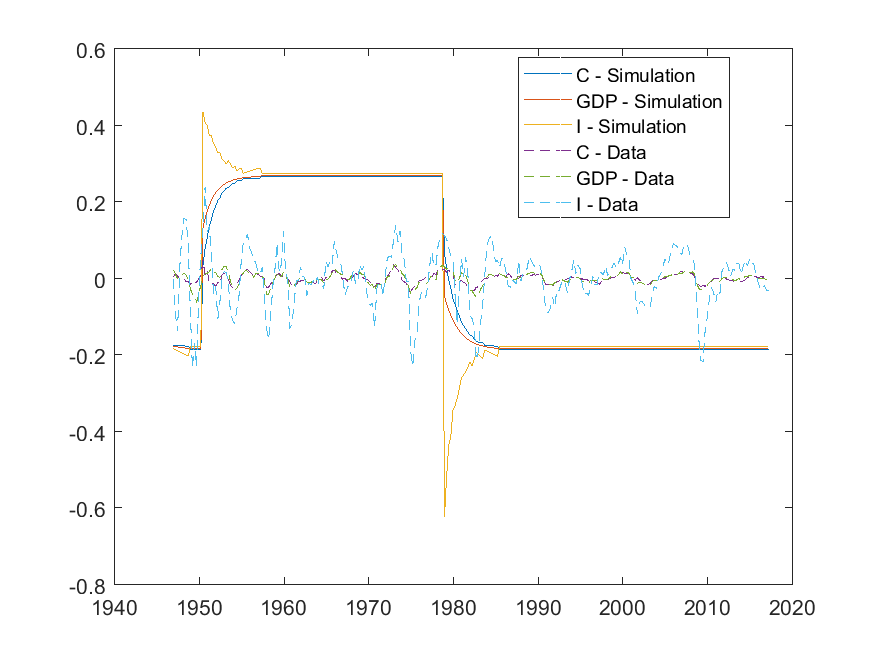
\includegraphics[width=\linewidth]{plot_sim}
		\caption{Simulation of RBC Model}
		\label{fig:plotsim}
	\end{figure}

	\begin{figure}[H]
	\centering
	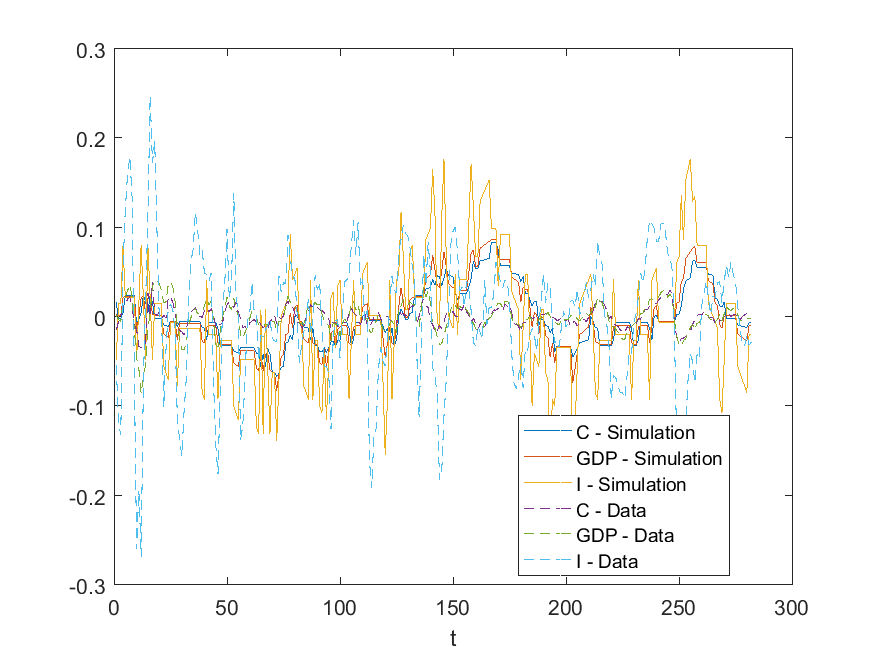
\includegraphics[width=\linewidth]{plot_sim_ex}
	\caption{Simulation of RBC Model}
	\label{fig:plotsimex}
\end{figure}
\end{enumerate}


\section*{Problem 3}
\begin{enumerate}[1.]
	\item 
	\underline{Sequential Problem}
		\begin{align*}
	\max &\sum_{t=0}^{\infty} \beta^t U(c_t,C_t) \\
	\st & C_t = F(K_t,N_t) + (1-\delta)K_t - K_{t+1}\\
	& c_t = C_t\\
	& K_{0} \text{ given.}
	\end{align*}
	
	Note that the households will maximizes utility when $N_t=1$, thus we can write $F(K_{t},1) = f(K_t)$.
	
	\underline{Recursive Problem}
	\begin{align*}
	V( K_{t}) = \max_{0\leq  K_{t+1} \leq f(K_t) + (1-\delta)K_t}  & \left\lbrace u( f(K_t) +  (1-\delta)K_t - K_{t+1},f(K_t) +  (1-\delta)K_t - K_{t+1}) + \beta V(K_{t+1})\right\rbrace 
	\end{align*}
	\item 
	
	\begin{enumerate}[(1)]
		\item First-Order conditions.
		
			\begin{align*}
			-u_1(C_t,C_t) - u_2(C_t,C_t) + \beta V'(K_{t+1})=0
			\end{align*}
	where $C_t=f(K_t) +  (1-\delta)K_t - K_{t+1}$
		
		\item Envelope conditions.
			\begin{align*}
			V'(K_t)=u_1(C_t^*,C_t^*)f'(K_t) +  u_2(C_t^*,C_t^*)f'(K_t)
			\end{align*}
			where $C_t^*=f(K_t) +  (1-\delta)K_t - g(K_{t})$ and $g(\cdot)$ is the policy function.
\end{enumerate}

\underline{Euler equation}
\begin{align*}
	&u_1( f(K_t) +  (1-\delta)K_t - g(K_t),f(K_t) +  (1-\delta)K_t - g(K_t)) \\
	&+ 
	u_2( f(K_t) +  (1-\delta)K_t - g(K_t),f(K_t) +  (1-\delta)K_t - g(K_t)) \\
	&=
	\beta \left[  u_1( f(g(K_t)) +  (1-\delta)g(K_t) - g(g(K_t)),f(g(K_t)) +  (1-\delta)g(K_t) - g(g(K_t)))\right.  \\
	&+
	\left. u_2( f(g(K_t)) +  (1-\delta)g(K_t) - g(g(K_t)),f(g(K_t)) +  (1-\delta)g(K_t) - g(g(K_t)))\right] 
	f'(g(K_t))
\end{align*}
or
\begin{align*}
u_1(C_t^*,C_t^*)+ u_2( C_t^*,C_t^*)
&=\beta \left[  u_1(C_t^{**},C_t^{**})+ u_2(C_t^{**},C_t^{**}) \right] f'(g(K_t))
\end{align*}
where $C_t^{*}=  f(K_t) +  (1-\delta)K_t - g(K_t)$ and $C_t^{**}=f(g(K_t)) +  (1-\delta)g(K_t) - g(g(K_t))$.

	\item 
	
	\underline{Sequential Problem}
			\begin{align*}
	\max &\sum_{t=0}^{\infty} \beta^t U(c_t,C_t) \\
	\st & c_t = F(K_t,N_t) + (1-\delta)K_t - K_{t+1}\\
	& K_{0}, C_t\text{ given.}
	\end{align*}
	
	Note that the households will maximizes utility when $N_t=1$, thus we can write $F(K_{t},1) = f(K_t)$. Moreover, in this setting the households are taking $C_t$ to be given.
	
	\underline{Recursive Problem}
	\begin{align*}
	V( K_{t}) &= \max_{0\leq  K_{t+1} \leq f(K_t) + (1-\delta)K_t} \left\lbrace u( f(K_t) +  (1-\delta)K_t - K_{t+1},C_t) + \beta V(K_{t+1})\right\rbrace 
	\\
	&\text{ where } C_t \text{ given}
	\end{align*}
	\item 
	
	\begin{enumerate}[(1)]
		\item First-Order conditions.
		
		\begin{align*}
		-u_1(f(K_t) +  (1-\delta)K_t - K_{t+1},C_t)+ \beta V'(K_{t+1})=0
		\end{align*}
		where $C_t=f(K_t) +  (1-\delta)K_t - K_{t+1}$.
		
		\item Envelope conditions.
		\begin{align*}
		V'(K_t)=u_1(f(K_t) +  (1-\delta)K_t - g(K_{t}),C_t^*)f'(K_t)
		\end{align*}
		where $C_t^*=f(K_t) +  (1-\delta)K_t - g(K_{t})$ and $g(\cdot)$ is the policy function.
	\end{enumerate}
	
	\underline{Euler equation}
	\begin{align*}
	&u_1( f(K_t) +  (1-\delta)K_t - g(K_t),f(K_t) +  (1-\delta)K_t - g(K_t)) \\
	&=
	\beta \left[  u_1( f(g(K_t)) +  (1-\delta)g(K_t) - g(g(K_t)),f(g(K_t)) +  (1-\delta)g(K_t) - g(g(K_t)))\right] f'(g(K_t))
	\end{align*}
	or
	\begin{align*}
	u_1(C_t^*,C_t^*)
	&=\beta \left[  u_1(C_t^{**},C_t^{**}) \right] f'(g(K_t))
	\end{align*}
	where $C_t^{*}=  f(K_t) +  (1-\delta)K_t - g(K_t)$ and $C_t^{**}=f(g(K_t)) +  (1-\delta)g(K_t) - g(g(K_t))$.
	

	\item
	
	Note that the social planner solution is different than the unique competitive equilibrium if $u_2(\cdot)\neq0$. 
	
	Since the social planner has more information than the household (it understands how the household impact the aggregate outcome), the utility generated from the social planner problem is going to be higher than the competitive equilibrium. 
	
	Hence, the competitive equilibrium is not Pareto efficient.
\end{enumerate}


\section*{Code}
\subsection*{Problem 2}
\lstinputlisting[language=Matlab]{value_function_ite.m}
\subsubsection*{Transition Matrix (tauchen.m)}
\lstinputlisting[language=Matlab]{tauchen.m}
\subsubsection*{Markov Chain (markovchain.m)}
\lstinputlisting[language=Matlab]{markovchain.m}
\subsubsection*{Value Function Iteration (bellman.m)}
\lstinputlisting[language=Matlab]{bellman.m}

\end{document}
